\chapter{Website}
\section{Features}
In this project, the only objective of the website was to collect information from the user, and stock them in the database.

When a user went for the first time on the website, he have to sign up, so we can collect informations about the company. After this operation he can access to his control panel where he can:
\begin{itemize}  
\item Create or edit their switchboard
\item Manage operators (the operator are people who will receive the call from the switchboard)
\item Manage the Company's informations
\end{itemize}  





\section{MVC}
The website is based on the Spring technologie,  it follow the MVC rule (Model-View-Controler). the view is separated from the controller and the model.

\begin{itemize}  
\item The view are the static web pages, in HTML and CSS, with pebble there are in .twig files
\item The controllers are files, coded in Java, which send data to the view
\item The model is like a kernel, he stock the informations, process them...

\end{itemize}  

Here is a schematic representation of the website architecture

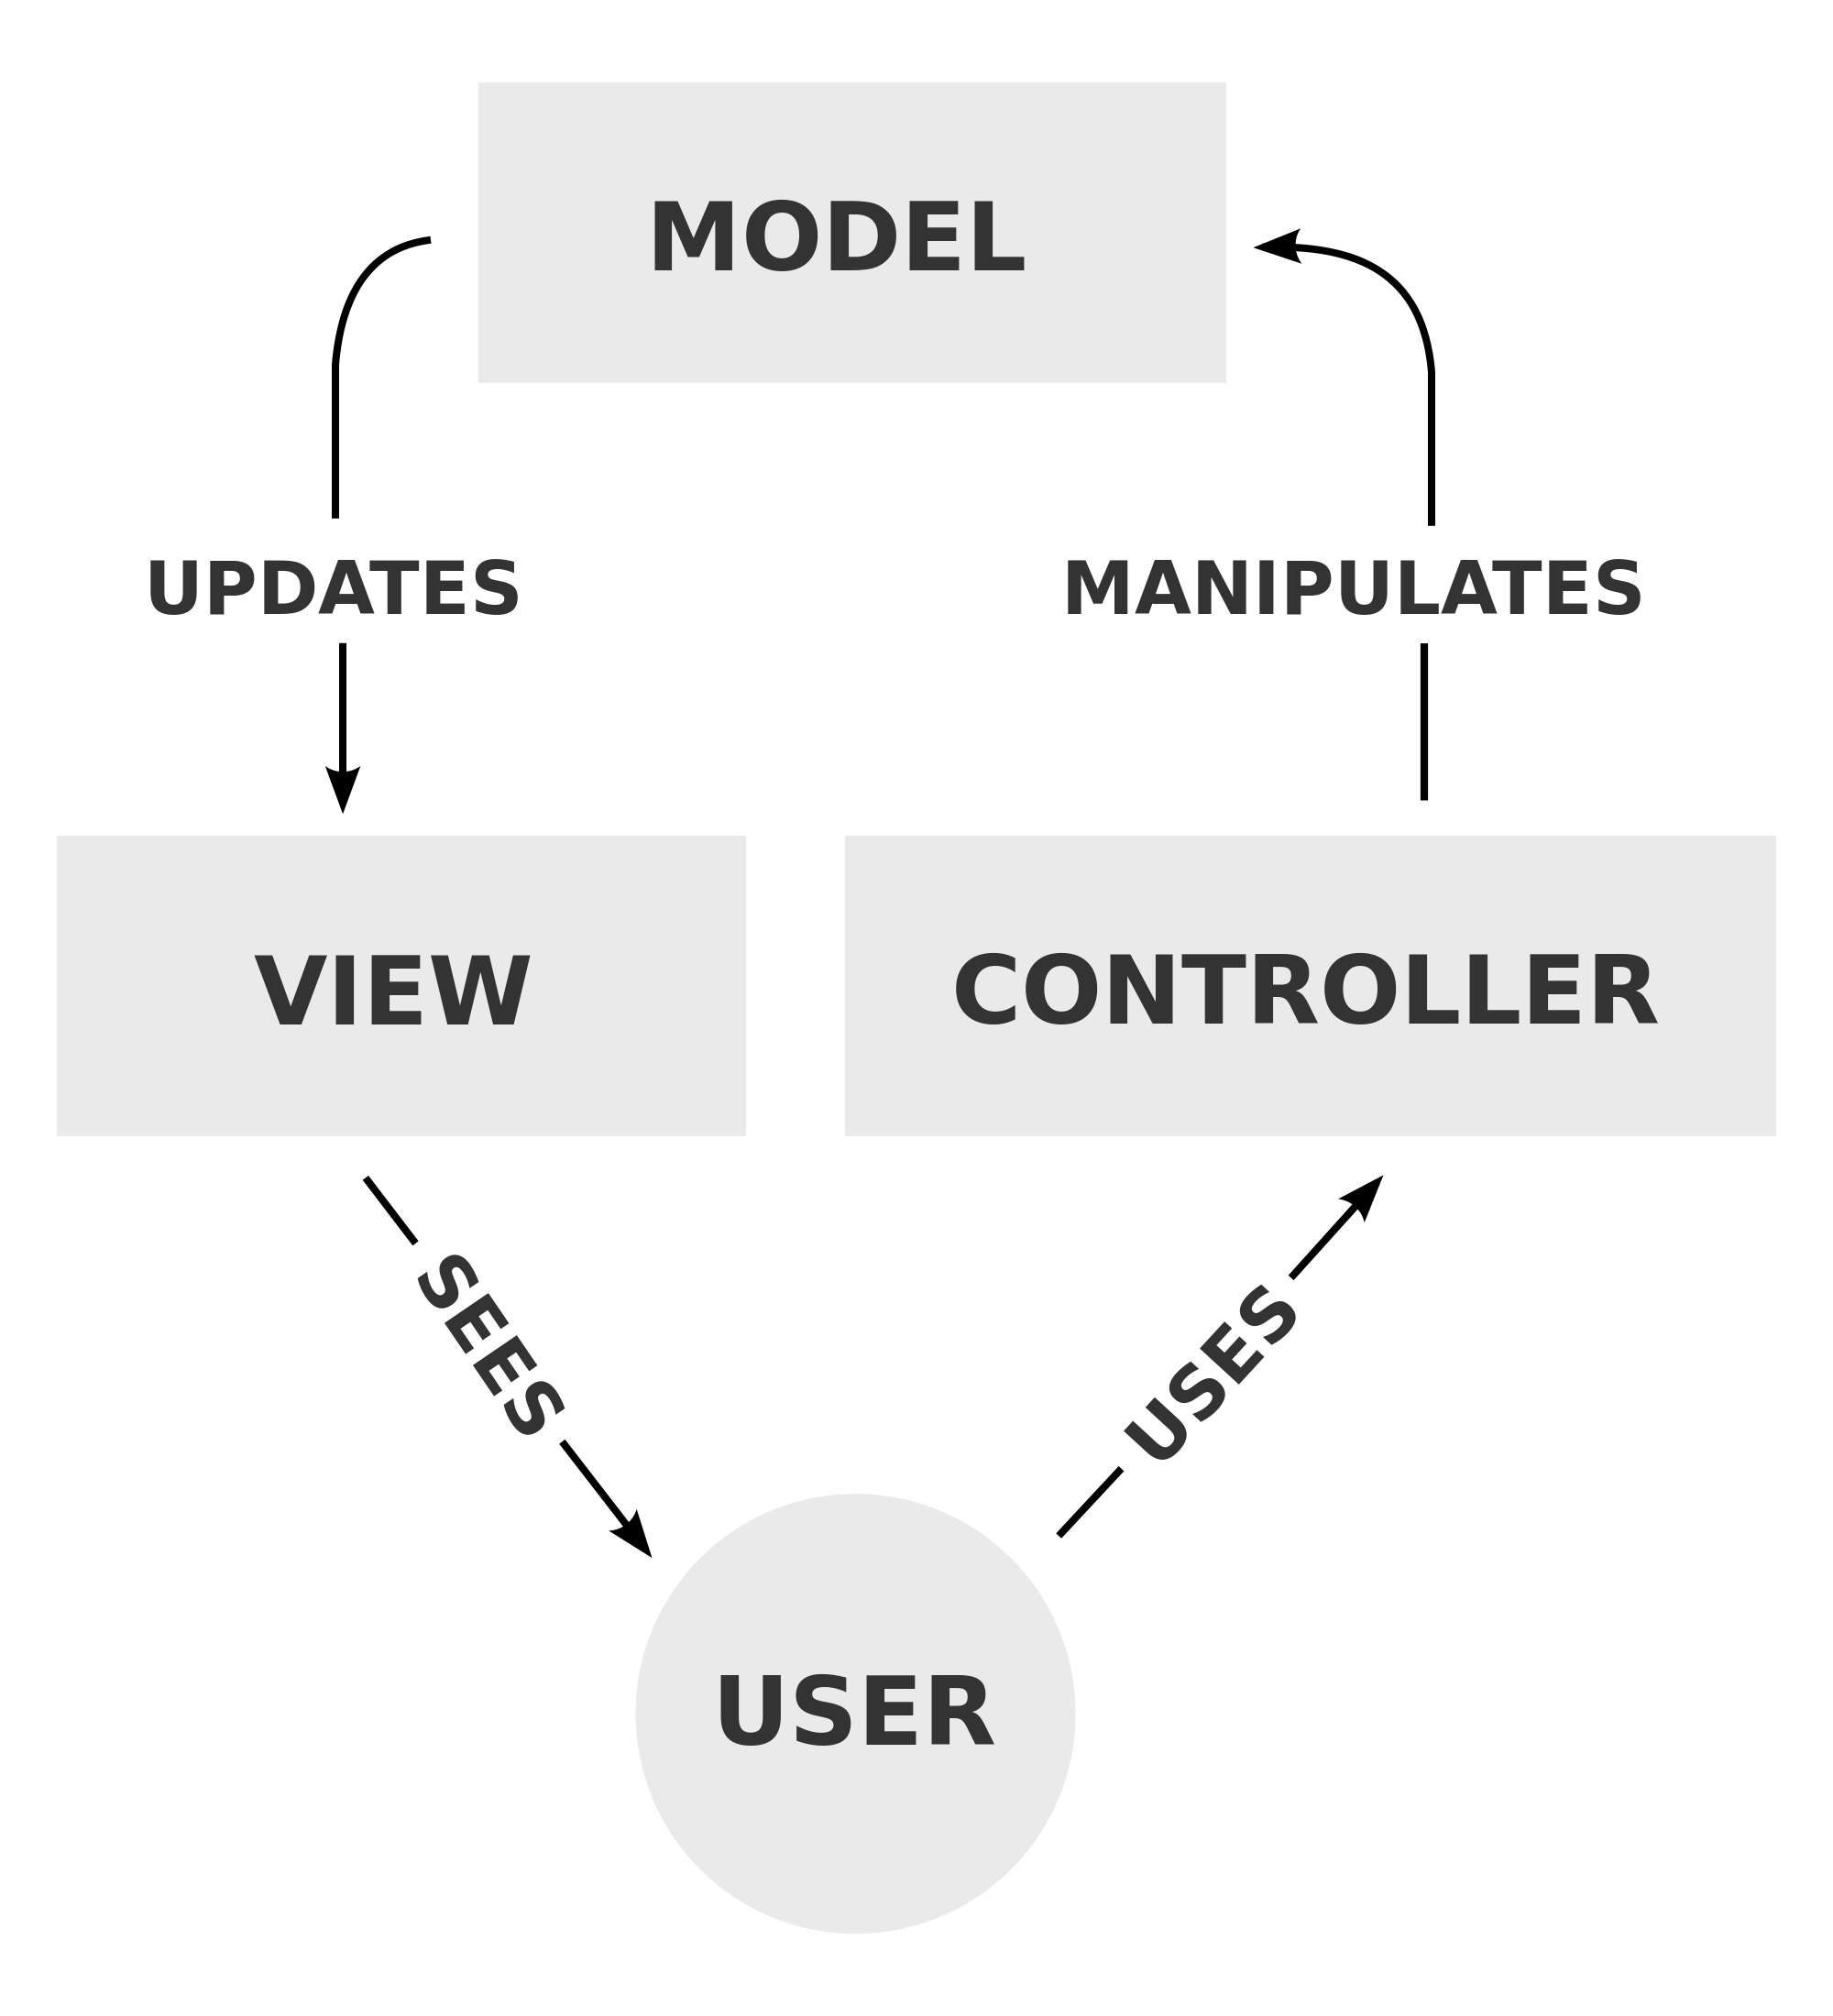
\includegraphics[width=0.50\textwidth]{img/mvc.png}




\section{DAO}

The DAO are the link between the program and the database. There are managed by the Hibernate technologie, coded in java.
In fact, we have one DAO per entity (switchboard, company...), those files contains functions which returns informations from the database.
\\
\\
Hibernate simplify the interaction with the database, we don't have to use standard SQL interaction.
It works with java object and an hibernate session, we use annotation in the Java class to describe the reproduction of this object in the database,
and we can manipulate this object, transfer it by the session and it will be save on the database.

\section{Services}

We have an other types of files calls "Services", it works with the DAO files.
Their role are to check data send from the application to the DAO, it's avoid errors in the datatbase.
For example it can check data receive from form.


\section{.twig}

The .twig files are an evolution of the HTML files, there are managed by pebble and represents the view of the website.
A .twig file can represent a file, or a part of a file (a layout), like a that we don't have to code every time the same code (like the menu...)
.twig offer something more than a classical html file, it allow to use Java object inside the view, so we can transfer a list and process it directly inside the view.


\section{Design}

Due to our inability to make a real design, we choose to take one from the internet
\\
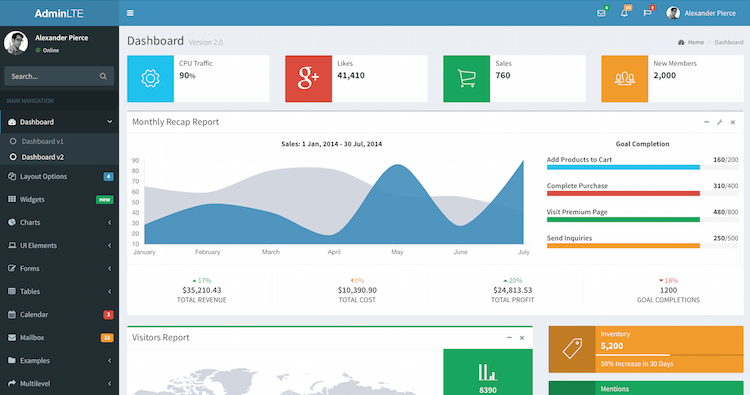
\includegraphics[width=0.70\textwidth]{img/design.png}
\\
We clear and and adapt it to our website.
This template is based on the Bootstrap framework which ease the front-end development of a website. Furthermore it a applies a responsive design which mean that our website will be functional on every platform (phone, tablets, computer...)









